\chapter{Cosmological probes}

\dots

\section{Cluster number counts}

\subsection{Structure formation}

\subsubsection{Spherical collapse model}

\subsection{Galaxy clusters}

The abundance and spatial distribution of galaxy clusters are sensitive to the growth rate of cosmic structures and expansion history of the Universe.

$$
S_8 = \sigma_8( \Omega_m / 0.3)^{0.5}
$$

where $\sigma_8$ is the amplitude of the matter power spectrum and $\Omega_m$ is the present-day matter density.

\subsection{The halo mass function}

The cluster abundance can be expressed as:
$$
\frac{dN}{dz d\Omega} = \frac{dV}{dz d\Omega} n(M, z)
$$
where the first term represents the geometry (comoving volume element) and the second term $n(M,z)$ represents the growth of structure.

The halo mass function is given by:
$$
n(z, M) = \frac{\rho_m}{M} f(\sigma) \frac{d \ln \sigma^{-1}}{dM}
$$

The variance of the density field is:
$$
\sigma(z, R) = \frac{1}{2\pi^2} \int_0^{\infty} dk \, k^2 P_m(z, k) |W(kR)|^2
$$
where $P_m(z,k)$ is the matter power spectrum.

The halo mass function depends on cosmological parameters: increasing $\Omega_m$ or $\sigma_8$ shifts the mass function to higher abundances. Cluster counts as a function of redshift show sensitivity to these parameters, with different combinations of $\Omega_m$ and $\sigma_8$ producing distinct predictions for the number of clusters observed at different redshifts.

\subsubsection{Massive neutrinos}

\textbf{Massive neutrinos} are produced in the early Universe and kept in thermal equilibrium by weak interactions.

Decoupling occurs at $T_{dec} \approx 2-4$ MeV, when $T_{dec} \gg m_\nu$, meaning neutrinos are ultra-relativistic at decoupling.

The free-streaming length is given by:
$$
\lambda_H \sim \frac{c}{H} = R_H \sim ct
$$

At this stage, neutrinos contribute to the \textbf{radiation} energy content.

The redshift of the \textbf{non-relativistic transition} is:
$$
(1 + z_{nr}) = \frac{1}{a_{nr}} \approx 2 \times 10^3 \left( \frac{m_\nu}{1 \text{ eV}} \right)
$$

The free-streaming wavenumber is:
$$
k_{nr} = 2\pi \frac{a_{nr}}{\lambda_h} = 0.018 \Omega_m^{1/2} \left( \frac{m_\nu}{1 \text{ eV}} \right) h \text{ Mpc}^{-1}
$$

After the non-relativistic transition, neutrinos contribute to the \textbf{matter} energy content.

The evolution of the free-streaming wavenumber $k_s = 2\pi \frac{a}{\lambda_s}$ shows three distinct regimes:
\begin{itemize}
    \item Free streaming regime (small scales, high $k$)
    \item Growth regime (intermediate scales)
    \item Super horizon regime (large scales, low $k$)
\end{itemize}


Neutrinos are diffused becouse of the free streaming wavelegth, so they are not clustered. They:

\begin{itemize}
    \item Delay the epoch of matter-raadiation equality
    \item Suppresses the growth of density fluctuation on scale smaller than the free streaming length
\end{itemize}

The higher the neutrino mass, the more they suppress the growth of density fluctuations, and the less massive objects are formed.

\subsubsection{Modified gravity}

There are many classes og mg models, e.g. $f(R)$:

$$
S = \dfrac 1{16 \pi G} \int \sqrt{-g} \lfloor R + f(R) \rfloor d^4 x
$$

Give rise to accelerated expansion and enhance gravity, therefore the growth rate of structures is increased.

Introduce screening mechanism that restores GR in high density environments: for object with mass above a given threshold, we restore the ... model.

% todo: add picture of Relative effect on the Halo Mass Function compared to ACDM

The halo mass function $n(z, M) = \frac{\rho_m}{M} f(\sigma) \frac{d \ln \sigma^{-1}}{dM}$ contains the factor $f(\sigma)$, which is a "universal" function:
\begin{itemize}
    \item Press \& Schechter (1974): approximated from spherical collapse of Gaussian density field
    \item Improved modeling using ellipsoidal collapse, e.g. Sheth \& Tormen (1999)
    \item Nowadays calibrated against N-body simulations
\end{itemize}

The calibration of $f(\sigma)$ depends on different factors:
\begin{itemize}
    \item Specifics of the simulation (e.g. box size, number of particles, softening length)
    \item Halo finder (e.g. linking length, FoF, SO)
    \item Mass definition (e.g. $M_{200,m}$, $M_{500,c}$)
    \item Redshift dependence
    \item Cosmological model (e.g. $\Lambda$CDM, wCDM, massive neutrinos)
\end{itemize}

\subsubsection{Baryonic effects}

Baryonic feedback (radiative cooling, star formation, AGN feedback) redistribute and expel mass from galaxy clusters.

baryonic feedback is most effective in the inner the regions of the halo and in low mass systems: the potential well is shallower, so the gas can escape more easily.

\section{From theory to observation}

Masses are not directly observable. Galaxy clusters are selected according to different observables (e.g. Richness, X-ray luminosity / photon counts, SZ signal), in general relarted to the observational techniqye, which correate with the mass.

Individual mass measurements are expensive and not feasible for cluster survey. We need to rely on mass proxies which are tightly correlated with the halo mass. We introduce an "Observable-mass relation".

Cosmological and scaling relation parameters are in general highly degenerate, and follow-up data are necessary to constrain simultaneously cosmology and the observable-mass relation. We need to combine cluster abundance and cluster mass estimates data to simultaneously constrain cosmology and the observable-mass relation(s).

\subsection{Cluster detection}

\subsubsection{Photometric survey}

Detection methods:
\begin{itemize}
    \item Overdensity of (red-sequence) galaxies
    \item Lensing effect
\end{itemize}

Observable/Mass proxy:
\begin{itemize}
    \item Richness (\# member galaxies)
    \item Luminosity
    \item Lensing signal
    \item Velocity dispersion (with spectra)
\end{itemize}

% todo: add z-$\lambda$ distribution of redMaPPer clusters in DES Y1

\subsubsection{X-ray survey}

Detection methods:
\begin{itemize}
    \item Extended X-ray sources
\end{itemize}

Observable/Mass proxy:
\begin{itemize}
    \item $L_X$ (X-ray luminosity)
    \item $T_X$ (temperature)
    \item Flux
    \item $Y_X = M_{gas} T_X$ (gas thermal energy)
\end{itemize}

X-ray emissivity from bremsstrahlung radiation of the ICM:
$$
\epsilon_\nu = \frac{dL}{dVd\nu} \propto n_e^2 g(\nu, T) T^{-1/2} \exp(-h\nu / k_B T)
$$

X-ray surveys are flux limited samples and not very sensitive to projections.

% todo: add X-ray images of clusters from eROSITA
% todo: add $L_X$-z distribution of X-ray selected catalogs

\subsubsection{SZ survey}

Detection methods:
\begin{itemize}
    \item Thermal Sunyaev-Zel'dovich effect (mm-wavelength)
\end{itemize}

Observable/Mass proxy:
\begin{itemize}
    \item SZ signal
\end{itemize}

The Compton-y parameter:
$$
y = \int d\ell \frac{k_B T_e}{m_e c^2} n_e \sigma_T
$$

The SZ signal is redshift independent, making it particularly useful for detecting clusters at high redshift.

% todo: add SZ spectral distortion plot
% todo: add mass and redshift distribution of SZ-selected cluster catalogs

\subsection{Cluster catalogs at different $\lambda$s}

% todo: listen the lecture, then enhance this section

ICM-selected (X-ray, SZ):
\begin{itemize}
    \item Mass limit $M \sim 2 \cdot 10^{14} M_\odot$
    \item Clean selection function (SZ signal independent of redshift!)
    \item Need optical follow-up for confirmation, redshift and WL data
\end{itemize}

Optically-selected:
\begin{itemize}
    \item Lower mass limit $M \sim 5 \cdot 10^{13}$
    \item $M_\star$ ($\times 10$ sample size)
    \item Selection function harder to model
    \item WL and photo-z data readily available
\end{itemize}

% todo: add $M_{500}$ vs redshift comparison plot for different surveys (eRASS1, Planck SZ, SPT-SZ, SPT-3G, SDSS, DES Y1, Euclid)

\subsubsection{Mass measurements from X-ray data}
\dots

\subsubsection{Mass measurements from spectroscopic data}

Assumimg spherical symmetry and dynamical equilibrium, we can dynamically estimate the mass using the Jeans equation:
$$
M(<r) = -\frac{r \sigma_r^2}{G} \left( \frac{d \ln \sigma_r^2}{d \ln r} + \frac{d \ln n_{\text{gal}}}{d \ln r} + 2\beta \right)
$$
where $\sigma_r$ is the radial velocity dispersion, $n_{\text{gal}}$ is the galaxy number density, and $\beta$ is the velocity anisotropy parameter.

% todo: add plot "Dynamical mass measurements in Euclid"

\subsubsection{Mass measurements from imaging}

The gold standard to perform mass validation on clusters is using the lensing signal.

The deflection does not depend on the dynamical state of the cluster.

we deal with two different regimes:
\begin{itemize}
    \item \textbf{Strong lensing}: Strong lensing regime in cluster's core ($\sim$ few hundred kpc). Deflection of the light is large enough to create multiple images of the same source and arcs $\rightarrow$ Precise measurements of the projected mass in scales enclosed by arcs. The mass reconstruction rely on assumptions on lens geometry and mass model $\rightarrow$ introduce systematic uncertainties of $\sim 10-20\%$.
    
    \item \textbf{Weak lensing}: At larger radii ($R > 300$ kpc), the tidal gravitational field causes subtle distortion of the shape of background galaxies -- weak lensing regime -- resulting in a coherent alignment of the sources. We can reconstruct the projected density profile by measuring the mean tangential shear profile at different radii around the cluster:
    $$
    \gamma_t(r_\perp), \Sigma(R) \Rightarrow \bar{\Sigma}(R) = \int d^2x \Delta\rho\left(\sqrt{R^2 + x^2}\right)
    $$
    To infer the mass profile one need to assume a parametric form for the halo density profile (e.g. NFW, Einasto profiles; Navarro+97, Einasto 1965) and correlated structures (2-halo term). In wide-field surveys, the weak lensing signal of clusters is usually stacked to increase the signal-to-noise and reduce the effect of shape noise and projection systematics, enabling calibration of the mass--observable scaling relation across large cluster samples.
\end{itemize}

% todo: add plot for mass measurement from imaging using different methods with high quality data 

\subsubsection{CMB cluster lensing}

The CMB provides a unique source of lensing signal at very high redshift ($z \approx 1100$), offering a powerful tool for cluster mass calibration that is independent of optical weak lensing systematics.

The CMB has intrinsic temperature anisotropies from the last scattering surface. When CMB photons pass through a galaxy cluster, they are deflected by the gravitational potential of the cluster. This deflection causes the CMB temperature gradient to appear shifted, creating a \textbf{dipole-like distortion} pattern aligned with the local CMB gradient direction. The amplitude of this dipole is proportional to the cluster mass and the magnitude of the background CMB gradient.

The distortion is quite small ($\sim 10$ µK for a $10^{15} M_\odot$ halo), but can be detected through stacking analysis of many clusters. By stacking the CMB signal around large samples of clusters (e.g., thousands of optically-selected clusters from surveys like redMaPPer), the signal-to-noise can be significantly enhanced, enabling robust mass calibration.

CMB lensing signal can also be detected in polarization data:
\begin{itemize}
    \item CMB Polarization (E-modes) provides a "cleaner" signal than temperature $\rightarrow$ Less contaminated by astrophysical foregrounds (e.g., tSZ effect, point sources)
    \item Recent results show $4.8\sigma$ detection of lensing signal from SPT-Pol data alone (Raghunathan+19)
\end{itemize}

% todo: add plot showing stacked 2D CMB lensing signal and azimuthally averaged convergence profile from CMB data around clusters (e.g., Baxter+19)
% todo: add figure showing example lensing dipole signal from simulated Q/U stacks and rotated background-subtracted Q and U stacks from SPT-Pol data

\subsubsection{Scaling relations}

Different detection techniques imply different mass proxies, mass calibration and systematics.  
The calibration of the observable-mass relation(s) requires:
\begin{itemize}
    \item Well defined selection function(s)
    \item A model to describe the parent distribution as a function of mass (halo mass function)
    \item A model to describe the PDF of the multivariate observable space: $P(\mathcal{X},\mathcal{O}|\mathcal{M})$
\end{itemize}


\chapter{Lecture 30/03/2026}

% \dots

% c-M primary dependence: mass and redshift -> the concentration decreases with mass and redshift.

% \dots

Cores and Self-Interacting Dark Matter (SIDM):

\begin{itemize}
    \item A finite self-interaction cross-section leads to heat transfer between DM particles, transporting energy from the hotter outer regions inward and reducing the central dark matter density — transforming a cusp into a core.
    
    \item "small" Cross-sections of order $\sigma/m \sim 1$ cm$^2$/g are sufficient to produce kpc-sized cores, consistent with observations of low-surface-brightness galaxies and dwarf galaxies.
    
    \item If SIDM is universal, cores should exist in all dark matter halos, from dwarf galaxies to galaxy clusters — providing a testable prediction across a wide range of scales.
    
    \item Central DM densities in the core regime are expected to be of order $10^7$--$10^8$ $M_\odot$/kpc$^3$, significantly lower than the cusp densities predicted by collisionless CDM simulations.
    
    \item However, SIDM halos are not immune to baryonic effects: gas cooling and stellar feedback can deepen the gravitational potential and restore a cusp-like profile, partially erasing the SIDM core — making observational tests model-dependent.
\end{itemize}


The bullet cluster:

The offset between the EM and WL signal peaks, along with the shape of the shock wave, provide compelling evidence for the presence of dark matter; moreover it allows to place constraints on the dark matter cross-section

El Gordo:

El Gordo (ACT-CL J0102-4915) is one of the most massive high-redshift galaxy cluster systems known, located at $z \approx 0.87$. It is the result of a major merger between two massive clusters, making it an exceptional laboratory for studying dark matter properties.

Observations show significant spatial offsets between its three main components:
\begin{itemize}
    \item \textbf{Hot gas (X-ray)}: The intracluster medium, traced by X-ray emission, is shock-heated and spatially displaced due to ram pressure during the collision.
    \item \textbf{Galaxies}: The stellar component of member galaxies, which are effectively collisionless and pass through the merger relatively unimpeded.
    \item \textbf{Dark Matter}: Detected via gravitational lensing reconstruction, the DM distribution shows offsets from both the gas and galaxies.
\end{itemize}

There are multiple ways to study these kinds of merging systems. One approach is to compare DM mass density profiles from lensing reconstruction with hydrodynamical simulation outputs (e.g., Valdarnini 2025).

Self-Interacting Dark Matter (SIDM) constraints from El Gordo:
\begin{itemize}
    \item A cross-section of $\sigma_{\text{DM}}/m_X \sim 4$--$5$ cm$^2$/g successfully reproduces the observed offsets between galaxies and dark matter.
    \item However, this level of interaction causes the dark matter halos to develop \textbf{``cores''} (flat density centers) rather than the ``cusps'' (sharp peaks) predicted by standard NFW models and seen in observations.
    \item This tension between the offset constraints and the core/cusp problem highlights the complexity of using merging clusters to constrain SIDM models.
\end{itemize}

The shape/slope of the halo profile, especially in the inner regions, can be used to test several fundamental physics models, such as the nature of dark matter (e.g. warm vs cold, interacting DM) or GR tesrt.

\missing{slide 52}

Linear perturbations of the FLRW metric:
$$
ds^2= - \left(1 + \dfrac {2\Phi}{c^2}\right) c^2 dt^2 + a^2(t) \left(1-\dfrac{2\Psi}{c^2} \right) [dr^2 + r^2 d\Omega^2]
$$
(assuming a flat universe)

\begin{itemize}
    \item $\Phi$ perturbs the time-time part of the metric $g_{00}$. It controls the motion of slow, non-relativistiv particles, such as cluster galaxies.
    \item $\Psi$ perturbs the space-space part of the metric $g_{ij}$. It controls ...
\end{itemize}


\subsubsection{Gravitational redshift in galaxy clusters}

Light escaping a gravitational potential well is redshifted:
$$
z_{gr} = \nabla \Phi / c^2
$$

For cluster masses $\sim 10^{14} M_\odot$, we have $cz_{gr} \sim 10km/s$ which is very smaller than Doppler broadening ($\sim 1000 km/s$).

Galaxies near the cluster centre sit deeper in the potential well and are more redshifted, so the GR velocity shift $\Delta(R)$ is most negative at small $R$ and rises (less negative) toward the outskirts. In the rest frame of the brightest cluster galaxy (BCG), this manifests as a systematic blueshift of the velocity distribution centroid.

\chapter{Clustering}

we have seen the cluster counts as the first moment of the density field. Now we will see the second moment of the density field: the variance.

\section{Evolution of density perturbations}

In quantum theory we know that even in empty fields we have small quantum fluctuations, that average to zero.

stretching the fluctuations outside the horizon, they freeze and are converted into curvature perturbations. Different regions of the universe have different curvature perturbations.

gravity amplifies overdensities.

$$
\left[\delta\phi_k \longrightarrow \zeta_k \longrightarrow \delta_m(\mathbf{x})\right]
$$

\begin{figure}[H]
    \centering
    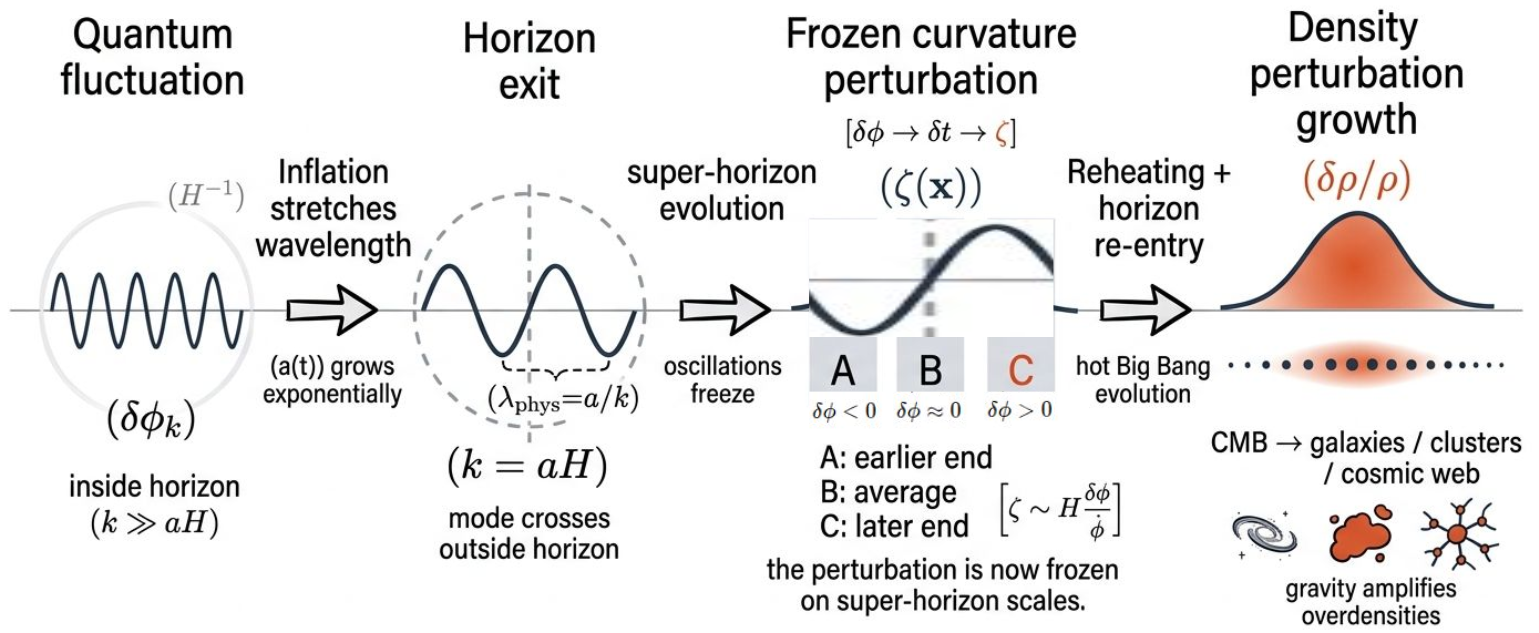
\includegraphics[width=0.9\textwidth]{assets/density-perturbations.png}
    \caption{Inflation stretches miscroscopic quantum fluctations to super-horizon scales, where they freeze as curvature perturbations and later seed the growth of cosmic structures.}
\end{figure}

The simplest models of inflation predict that the initial fluctuations constitute a Gaussian random field, with an almost purely adiabatic primordial perturbations with a near scale-invariant power spectrum. In these models the primordial power spectrum is often described in terms of a spectral index ns and an amplitude of the perturbations As as (k p = 0.05 Mpc-1 = pivot scale ):

$$
P(k) = A_s \left(\frac{k}{k_p}\right)^{n_s}
$$

\dots

The overdensity field is:

$$
\delta(x) = \dfrac{\rho (x) - \langle \rho \rangle}{\langle \rho \rangle}
$$

For the CDM model, we have:

\begin{table}[H]
    \centering
    \begin{tabular}{c|c|c}
        \toprule
        & $z > z_{eq}$ (RD) & $z < z_{eq}$ (MD) \\
        \midrule
        $R > R_H$ & $\delta_r \propto \delta_m \propto a^2$ & $\delta_r \propto \delta_m \propto a$ \\
        $R < R_H$ & $\delta_{cdm} \sim \text{const}$, $\delta_{b+\gamma}$ oscillations & $\delta_{cdm} \propto a$; $z < z_{rec}$: $\delta_b \rightarrow \delta_{cdm}$ \\
        \bottomrule
    \end{tabular}
\end{table}

Matter-radiation equality:

$$
\dfrac{\rho_m (a_{eq})}{\rho_r (a_{eq})} = 1 \qquad \qquad 1 + z_{eq} = \dfrac{a_0}{a_{eq}} \simeq 3250
$$

The Hubble radius is:

$$
R_H(a) = \dfrac{c}{H(t)} \sim c t
$$

The primordial power spectrum of density fluctuations gets “processed” by the growth of density perturbations:

$$
P(k, z) = P_{primordial}(k) T^2(k, z)
$$

where the transfer function $T(k)$ takes into account the effects of gravitational amplification of density perturbation mode of wavelength $k$

\textbf{Cosmic Relics}:
\begin{itemize}
    \item \textbf{Non-thermal Relics}: not producted in thermal equilibrium (TE) with the rest of the Universe
    \item \textbf{Thermal Relics}: are held in TE with other components of the Universe until they "decouple", which happens when interaction rate $\Gamma = n(\sigma v)$ drops below expansion rate $H(a)$.
    \begin{itemize}
        \item Hot Dark Matter: ...
        \item Warm Dark Matter: ...
        \item Cold Dark Matter: ...
    \end{itemize}
\end{itemize}

\missing{slide 10: above horizon, below horizon; slide 11: Baryonic Acoustic Oscillations}

\subsection{Two-point correlation function}

%todo: enhance this section

The two-point correlation function, $\xi(r)$, is the excess probability of finding two tracers at a given distance, compared to a random distribution:

$$
dP = n(\ + \xi(r) dV)
$$

if $\xi(r) = 0$, then the probability is simply given by the number of tracers per unit volume.

We have 2 correlation function estimators:
\begin{itemize}
    \item \textbf{Peebles-Hauser estimator}:
    $$
    \hat \xi(r) = \dfrac{DD(r) - RR(r)}{RR(r)}
    $$
    \item \textbf{Landy-Szalay estimator} (more unbiased):
    $$
    \hat \xi(r) = \dfrac{DD(r) - 2 DR(r) + RR(r)}{RR(r)}
    $$
\end{itemize}

Using the two-point correlation function we can characterize the different clustering properties between the distributions.

% todo: add plot of the two-point correlation function

Assuming the universe is isotropic, the correlation function is a function of a scalar distance. The two-point correlation function can then be written as:
$$
\xi(r) = \langle \delta(\vec x) \delta(\vec x + \vec r) \rangle
$$

The two-point correlation function is closely connected to the power spectrum, they form a fourier transform pair:
$$
\xi(\vec r) = \dfrac 1{(2\pi)^3} \int d^3 k P(\vec k) e^{i \vec k \cdot \vec r}
$$

$$
P(\vec k) = \int d^3 r \xi(\vec r) e^{-i \vec k \cdot \vec r}
$$

...
% todo: add considerations

\begin{figure}[H]
    \centering
    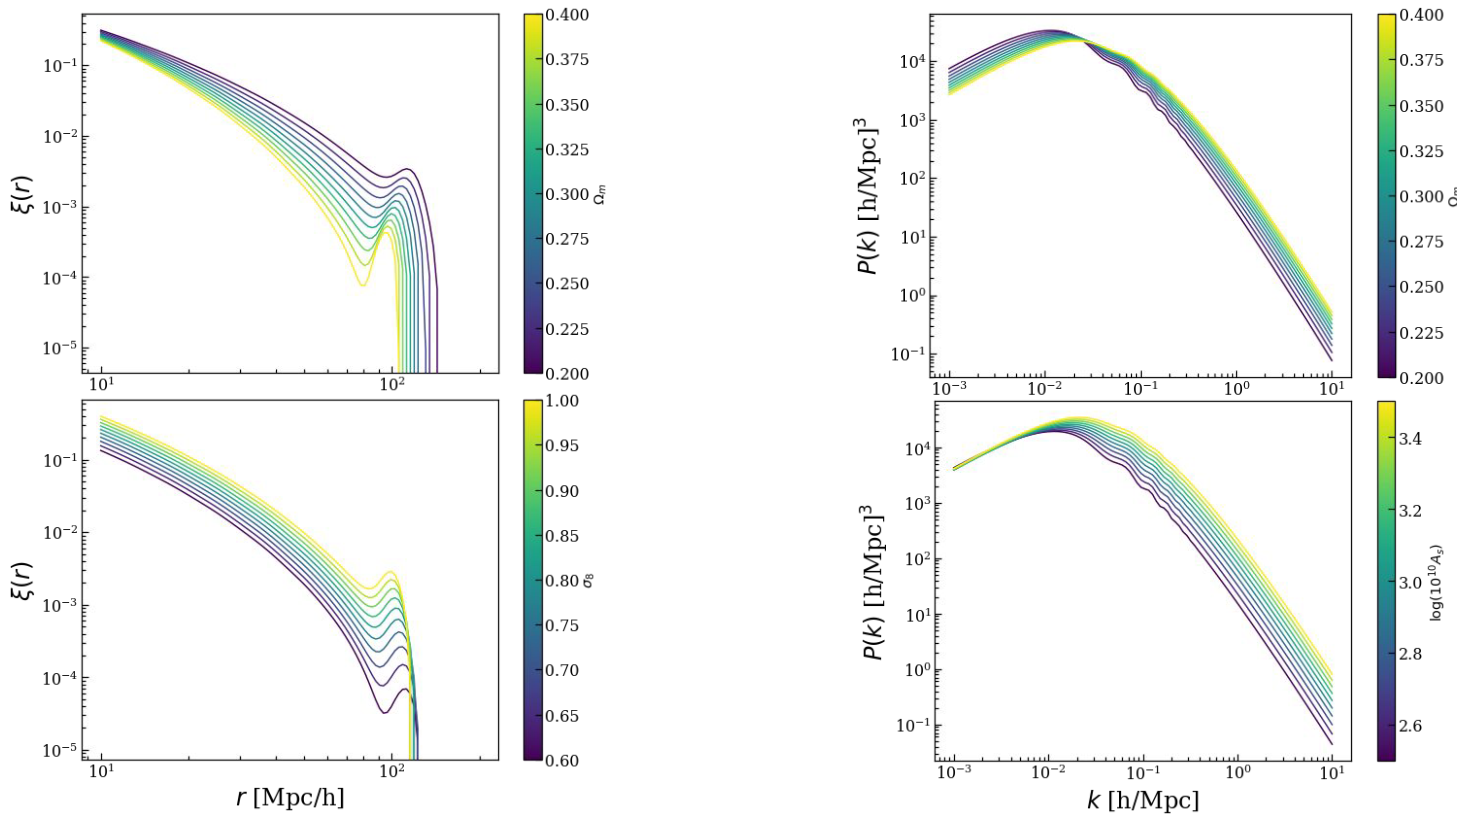
\includegraphics[width=0.6\textwidth]{assets/2pt-spectrum.png}
\end{figure}

\subsubsection{Non-linear evolution}

In the linear regime ($\delta \ll 1$) we can calculate the evolution of a density field using linear perturbation theory:
$$
P_{\text{Lin}}(k,z) = D(z) P_{\text{Lin}}(k,z=0)
$$

In the non-linear regime ($\delta > 1$) perturbation theory is no longer valid. \textit{Modes start to couple} to each other, and one can no longer describe the evolution of the density field with a simple growth rate: in general, no analytic solutions exist and we must rely on simulations.

\begin{observationblock}{Mode-coupling}
    Because of this mode-coupling, the density field loses its Gaussian properties, i.e., in the non-linear regime, we no longer have a Gaussian random field. Hence, higher-order moments are required to completely specify the density field.
\end{observationblock}

\subsection{Bias}

Halo formation is not a random process; haloes are not a Poisson sampling of the matter field. Rather, they only form where the (smoothed) density field has a sufficiently high value: the critical overdensity for collapse. This "threshold" causes haloes to be biased tracers of the mass distribution: Because of the modulation of the small-scale density field by the long-wavelength modes, overdense regions (on large scales) contain enhanced abundance of dark matter haloes, so that these haloes display enhanced clustering.

\dots

The collapsed structures we observe today, that is, galaxies and galaxy clusters, are formed at the locations of the peaks of the matter density field and more massive objects correspond to higher peaks. Thus, we expect their distribution to be a biased tracers of the underlying mass distribution and the bias grows with the mass of the objects.

$$
\delta_h = b_h \delta_m
$$

$$
\xi_{hh}(r) = \langle \delta_h(x) \delta_h(x + r) \rangle = b_h^2 \xi_{mm}
\qquad \xrightleftharpoons[\mathcal{F}^{-1}]{\mathcal{F}} \qquad
P_{hh}(k) = \langle \tilde \delta_h(k) \tilde \delta_h^*(k') \rangle = b_h^2 P_{mm}(k)
$$

Galaxy clusters, arising from the highest density peak of the matter density field, have the largest bias. Their bias can be predicted from theory (or calibrated from simulations) from the halo mass function:

On the other hand, forming on the rare high density peaks of the matter density field, galaxy clusters are a sparse tracer of $\delta_m$ , and their 2pt CF signal is largely disturbed by shot noise.

\subsubsection{Spectroscopic vs photometric surveys}

% todo: complete this section

\dots

\begin{minipage}{0.49\textwidth}
\begin{center}
\textbf{Spectroscopic survey}
\vspace{1em}
\end{center}
\begin{itemize}
    \item Accurate 3D reconstruction
    \item Medium depth
    \item Low density
    \item Strong selection effects
\end{itemize}
\end{minipage}%
\hfill
\begin{minipage}{0.49\textwidth}
\begin{center}
\textbf{Photometric survey}
\end{center}
\vspace{1em}
\begin{itemize}
    \item Low resolution along the line-of-sight
    \item Usually deeper and larger area (i.e. larger volume)
    \item High density
    \item ~ No selection effects
\end{itemize}
\end{minipage}

\dots

\subsubsection{Angular 2pt correlation function}

Instead of reconstructing the 3d power spectrum, we take bins and then we project them \dots


\section{Baryonic Acoustic Oscillations}

The clustering of matter encodes a preferred scale, \textit{the sound horizon at the baryon drag epoch} of the early universe. This feature, which is imprinted on the matter distribution of the early universe by physics around recombination and earlier, is stretched with the expansion of the universe, appearing at a comoving galaxy separation of $r_d \sim 150$ Mpc. Since galaxies trace the matter content of the universe, the BAO feature is transferred into galaxy clustering, where it manifests as a single localised peak in the galaxy correlation function and an oscillatory signature, or “wiggles”, in the galaxy power spectrum. The signature is also visible in other tracers of mass such as fluctuations in the Lyman-$\alpha$ forest — spectral features that indicate the radial distribution of neutral hydrogen clouds between the observer and distant quasars, as well as the CMB. Using BAO we can study the evolution of the Universe's geometry, thus test for dark energy dynamics and spatial curvature, and in combination with other probes constrain the Hubble constant, the sum of neutrino masses, and the number of light species.

\dots

\subsubsection{Angular diameter distance}

The turnover point occurs because of the expansion of the universe and the finite speed of light: very distant objects were closer to us when they emitted the light we see today. At that time they spanned a larger angle.

\dots

\subsubsection{Redshift space distortions}

Due to peculiar velocities (along the line of sight), the redshift
distances available from a galaxy redshift survey deviate from
the true, proper distances. This results in redshift space
distortions in the clustering measurements.

$$
v = v_{\text{exp}} + v_{\text{pec}} = H_0 d(z) + v_{\text{pec}}
$$

$$
z_{\text{obs}} = z_{\text{exp}} + \frac{v_{\text{pec}}}{c}(1 + z_{\text{exp}})
$$

\textbf{L.o.s. Proper Distance measured in redshift space:}

$$
s = \frac{v}{H_0} = d(z) + \frac{v_{\text{pec}}}{H_0}
$$

\begin{itemize}
    \item \textbf{Kaiser effect:}

    On large scales, peculiar velocities reflect the (linear) infall motions towards overdensities, causing a circle in real space to appear “squashed” in redshift space.

    \item \textbf{Finger-of-God effect:}

    On small scales, peculiar velocities are due to the nonlinear virialized motion of galaxies inside their host haloes, causing a circle in real space to appear “stretched” in redshift space.
\end{itemize}

\begin{figure}[H]
    \centering
    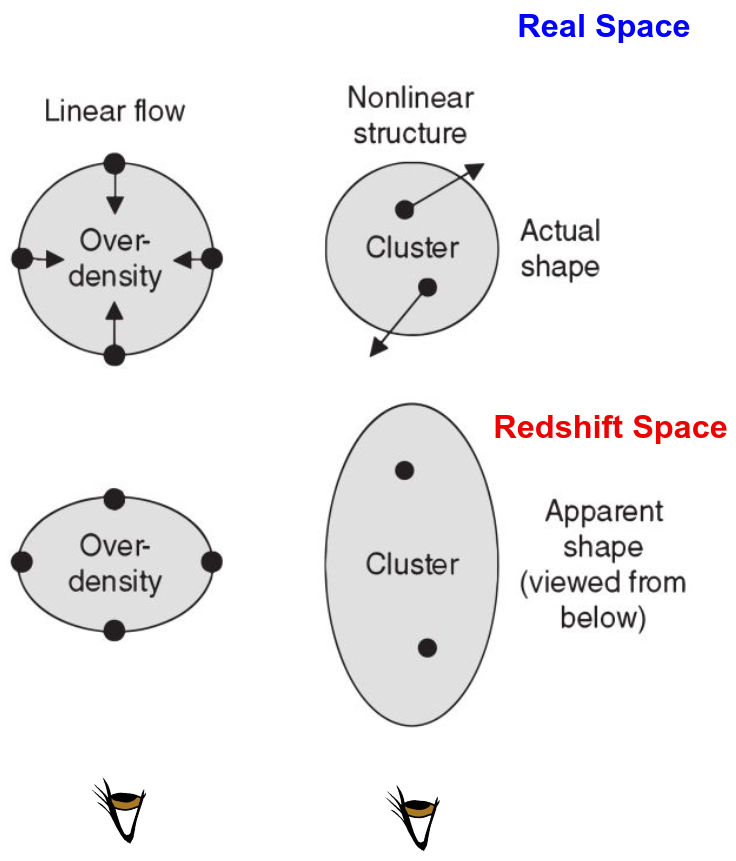
\includegraphics[width=0.6\textwidth]{assets/real_vs_redshift.png}
\end{figure}

Only radial distances are affected by Doppler shifts from peculiar velocities.  
The key point is that these peculiar velocities are generated by structure itself, so the clustering pattern measured in redshift space is systematically distorted with respect to real space. As a result, the galaxy two-point correlation function, isotropic in real space, becomes anisotropic in redshift space.

For a galaxy pair, define
$$
\mathbf{s} \equiv \mathbf{s}_1-\mathbf{s}_2, 
\qquad
\mathbf{l} \equiv \frac{\mathbf{s}_1+\mathbf{s}_2}{2},
$$
and decompose the separation into line-of-sight and transverse components:
$$
\pi \equiv \frac{|\mathbf{s}\!\cdot\!\mathbf{l}|}{|\mathbf{l}|},
\qquad
\sigma \equiv \sqrt{\mathbf{s}\!\cdot\!\mathbf{s}-\pi^2}.
$$
We then measure the anisotropic correlation function $\xi(\sigma,\pi)$.

In $\xi(\sigma,\pi)$ contour plots, small-scale elongation along the line of sight traces the Finger-of-God effect, while large-scale compression traces the Kaiser effect.

\dots

